
\documentclass[12pt]{article}
\setlength\parindent{0pt}
\usepackage{fullpage}
\usepackage[margin=0.5in]{geometry}
\usepackage{amsmath}
\usepackage{graphicx}
\setlength{\parskip}{4mm}
\def\LL{\left\langle}   % left angle bracket
\def\RR{\right\rangle}  % right angle bracket
\def\LP{\left(}         % left parenthesis
\def\RP{\right)}        % right parenthesis
\def\LB{\left\{}        % left curly bracket
\def\RB{\right\}}       % right curly bracket
\def\PAR#1#2{ {{\partial #1}\over{\partial #2}} }
\def\PARTWO#1#2{ {{\partial^2 #1}\over{\partial #2}^2} }
\def\PARTWOMIX#1#2#3{ {{\partial^2 #1}\over{\partial #2 \partial #3}} }
\newcommand{\BE}{\begin{displaymath}}
\newcommand{\EE}{\end{displaymath}}
\newcommand{\BNE}{\begin{equation}}
\newcommand{\ENE}{\end{equation}}
\newcommand{\BEA}{\begin{eqnarray}}
\newcommand{\EEA}{\nonumber\end{eqnarray}}
\newcommand{\EL}{\nonumber\\}
\newcommand{\la}[1]{\label{#1}}
\newcommand{\ie}{{\em i.e.\ }}
\newcommand{\eg}{{\em e.\,g.\ }}
\newcommand{\cf}{cf.\ }
\newcommand{\etc}{etc.\ }
\newcommand{\Tr}{{\rm tr}}
\newcommand{\etal}{{\it et al.}}
\newcommand{\OL}[1]{\overline{#1}\ } % overline
\newcommand{\OLL}[1]{\overline{\overline{#1}}\ } % double overline
\newcommand{\OON}{\frac{1}{N}} % "one over N"
\newcommand{\OOX}[1]{\frac{1}{#1}} % "one over X"



\begin{document}
\pagenumbering{gobble}
\Large
\centerline{\sc{Homework 7}}

\normalsize
\centerline{\sc{Due in recitation on Friday, April 8}}

\begin{enumerate}


\item{In the classic computer game {\it Portal}, the player is asked to solve
	puzzles with the use of a ``portal device''.
	

\begin{minipage}{0.4\textwidth}
	This device can create two connected portals
	on, for example, the floor and a wall. An object entering one portal with speed $v$
	will exit the other with the same speed. 
	The game's narrator helpfully explains that ``Forward momentum, a product of mass
	and velocity, is conserved between portals. In layman's terms: {\bf speedy thing
		goes in; speedy thing comes out.}''
	\end{minipage}
	\begin{minipage}{0.5\textwidth}
		\hspace{0.1\textwidth}
	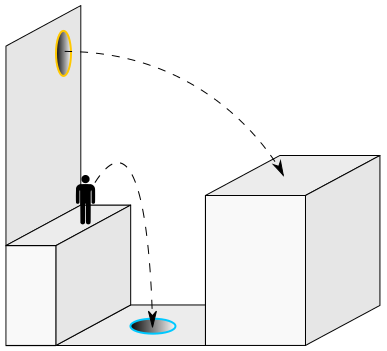
\includegraphics[width=0.8\textwidth]{Portal_physics-2.png}
\end{minipage}
	\begin{enumerate}
	\item Is this an accurate statement of the law of conservation of momentum? Does such a device conserve momentum, as the narrator states? If not, why not?
	
	\item Does this portal device conserve kinetic energy?
	
	\item Does it conserve {\it total} energy (kinetic plus potential)?
	\end{enumerate}
	
}

\bigskip

\item A person of mass 50 kg is ice-skating on a frozen lake with his dog Kibeth, who has a mass of 15 kg. He is skating due north at 3 m/s.

Kibeth realizes that he's carrying snacks in his pocket, and would like one for herself. (Or maybe she is just being friendly!) She runs after him and tackles him from behind and the side, knocking him down. The two of them collapse on the ice and begin to slide, as Kibeth tries to get the treats out of his pocket; they are moving at an angle 20 degrees west of north at 4 m/s.

What was Kibeth's velocity before she tackled him? {\it (Remember velocity is a vector.)}

\bigskip

\item Suppose that two small spacecraft, each with a mass of 2000 kg, are drifting next to each other. One of them has an astronaut on board; with her equipment, she has a mass of 200 kg. 

Both craft are moving in the $x-$direction at a velocity of $\vec v_i = (0.5~\rm m/\rm s, 0)$. An astronaut wants to travel from one to the other. She pushes off of one spacecraft and jumps onto the other craft; as she floats through the air, she travels in the $y-$direction with a velocity of $\vec v_a = (0, 1~\rm m/\rm s)$. Note that when she moves through the air, she is moving {\it only} in the y-direction.


\begin{enumerate}
	\item What will the velocity of the first spacecraft be after she jumps off of it? {\it (Velocity is a vector; you can give its components.)}
	
	
	\item What will the velocity of the second spacecraft be after she lands on it?
	
	
	\item Explain in words why the $y-$components of their final velocities are {\it almost} equal and opposite, but are not quite the same magnitude.
	
	\item Explain in words why the $x-$components of their final velocities are {\it almost} equal. 
\end{enumerate}

\bigskip

\item A forensics laboratory is investigating a crime and wants to measure how fast a particular gun shoots bullets. They don't have access to high-speed photography. All they have a clay block sitting on a table.

One of the detectives says ``Hey, we can figure it out using this! We'll set the block on a table and shoot a bullet into the block; the faster the bullet is going, the further the block will slide before it comes to a stop!''

Another detective says ``Yes, we can do that! In addition to how far the block slides on the table, we'll need to measure two things about the block and one thing about the bullet in order to figure it out.''

\begin{enumerate}
	\item What things must they measure to conduct the experiment?
	\item Determine a formula for the speed of the bullet in terms of the other things you measured.
\end{enumerate}

\item Drivers approaching the city of Denver, Colorado from the west travel on Interstate 70 as they descend from the Rocky Mountains (a tunnel at 3400 meters above sea level) into the city. 
\medskip

\begin{minipage}{3in}
Consider a section of this road that is 23 km long; drivers descend 800 meters in this distance. In this problem, you will consider the difficulties faced by truck drivers as they descend this section of road into Denver; as an example, consider a truck with a mass of 30,000 kg.

\end{minipage}
\begin{minipage}{4in}
\begin{center}
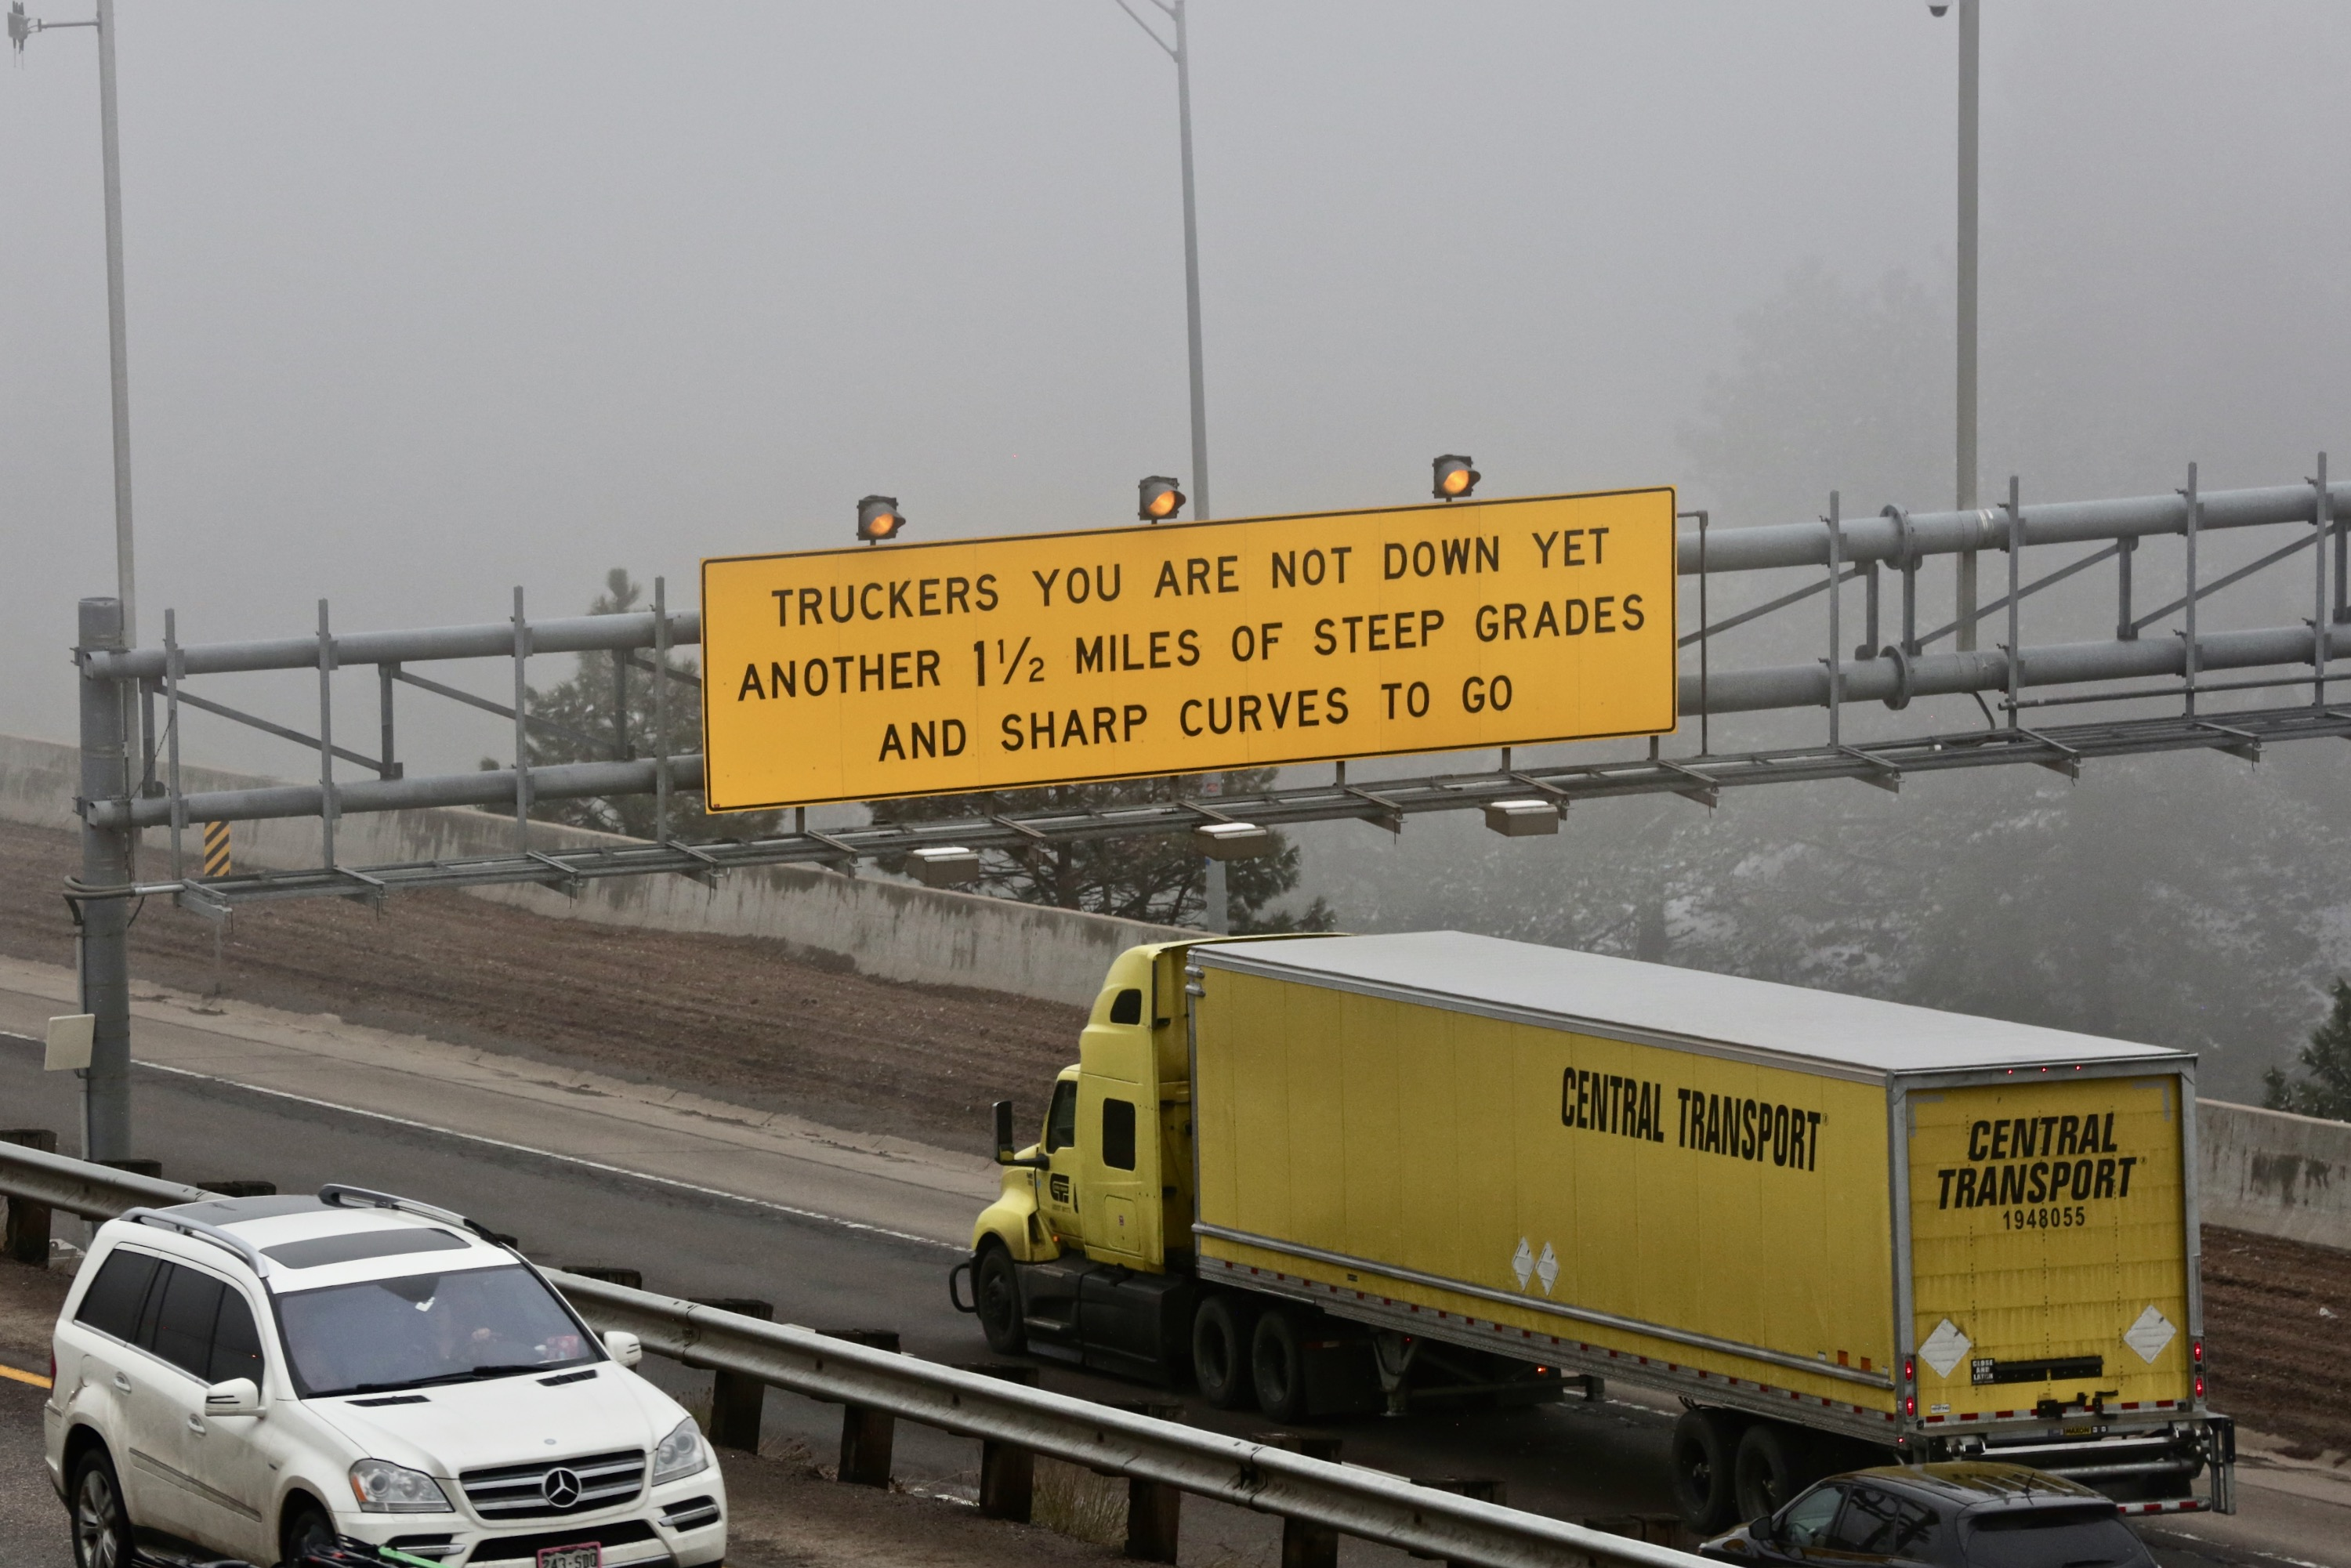
\includegraphics[width=3in]{trucker-sign.jpg}

\tiny \it Photo: Hart Van Denburg / Colorado Public Radio

\end{center}
\end{minipage}
\medskip



\begin{enumerate}
	\item Assuming a completely ideal situation in which the truck rolled freely down the slope with no interference from friction, how fast would the truck be traveling at the bottom of the slope. Convert this into km/hr or miles/hour; is this a reasonable thing for a truck driver to do?
	
	\item Thankfully, trucks are equipped with brakes which convert kinetic energy into heat through friction. This heat is then dissipated into the atmosphere. If a truck wants to maintain a constant speed down the hill, how much energy must its brakes absorb in total? (Compare this to the 270 MJ stored in the batteries of last week's Tesla.)
	
	\item Suppose a truck's brakes can dissipate heat at a rate of 250 kW. (If the driver tries to go faster than that, their brakes will heat up and lose effectiveness.) How fast could our driver go down this road safely? 
	
\end{enumerate}

\newpage


\item The top end of a spring with spring constant $k$ is attached to the ceiling; a mass $m$ hangs from the bottom (initially at rest). 

\begin{enumerate}
	\item How far below the spring's equilibrium point does the mass hang?
	\item A person attaches a second mass $m$ to the spring and releases it. When the mass is added, the extra weight stretches the spring out further,
	falling down an additional distance before the elastic force pulls it back up.
	
How far below the spring's equilibrium point do the masses fall before they start to come back up?

\item The masses bounce up and down for a while before eventually
coming to rest (due to air drag, friction, and the like).
Once they come to rest, how far below the equilibrium point
will they be located?
\end{enumerate}

{\it Hint: This problem is surprisingly nuanced. In each case, think very carefully about whether the net \rm{force} on the masses \it or their \rm{velocity} \it is zero.}
 
 \bigskip
 
\item A professor from Syracuse University's Department of Mad Science sees the Physics Department's rocket-powered car and decides to improve it. They increase the rocket thrust to $F_T$, put skis on the bottom (to suit the Syracuse winters), and take it out to the frozen surface of Lake Onondaga to test it. The rocket car along with the mad scientist have a mass of $m$. 

However, they accidentally leave their calculator in radian mode while assembling it, so the rocket instead exhausts its gas at an angle $\theta$ below the horizontal. (This means that the thrust force points forward and upward.)

The coefficient of kinetic friction between the ice and the skis is $\mu_k$.

They fire the rocket and travel forward along the ice. After traveling a distance $d$, they confirm that this will suffice for their mad-scientific purposes and shut down the rocket; they coast a further distance $b$ before coming to a stop.

\begin{enumerate}
	\item Write an expression for the work done by the force of friction during the entire motion.
	\item Write an expression for the work done by the thrust force during the entire motion.
	\item Show that the distance the sled coasts is 
	
	$$b=\frac{F_T d \cos \theta - \mu mgd + \mu d F_T \sin \theta}{\mu mg}.$$
	
	(Note that an earlier version of this homework set had an error in this equation.)
\end{enumerate}

\bigskip

\item Before they can test their rocket sled, however, they need to remove a boulder that is blocking the way. Being a mad scientist, they decide to blow it up.

They use a bit of dynamite to blast the rock into two pieces. The big piece has three times the mass of the little piece. Both slide along the ice (with the same coefficient of kinetic friction) before finally coming to a stop.

If the little piece slides 180 meters before coming to a stop, how far does the big piece slide?

{\it (It may seem like you don't have enough information to figure this out, but you do! This was a previous exam question.)}

 

\end{enumerate}
\end{document}
